% PROBABILISTIC UNCERTAINTY PROPAGATION
We now focus on probabilistic uncertainty propagation.
The goal is to quantify the influence of input parameter uncertainty on the predictions of an engineering model \cite{Uncertainty:Lee2009,Uncertainty:Arnst2014}.
By representing the uncertain inputs as random variables with a prespecified probability distribution, the problem becomes to characterize the corresponding output distribution.
% PROBABILITY/STATISTICS
After a short intermezzo with slightly more technical probability theory, only a basic familiarity with elementary statistics is required.
Introductions for an engineering target audience can be found in \cite{Statistics:Soong2004,Statistics:Benaroya2005,Statistics:Schwarzlander2011}.

\subsection{Engineering model}
% DETERMINISTIC MODEL
In the context of UQ, a \emph{model} of an engineering system is a mathematical representation or computational simulation of the relevant physical processes.
For given input parameters \(\bm{x} \in \mathcal{D}_{\bm{x}}\) from the domain \(\mathcal{D}_{\bm{x}} \subseteq \mathds{R}^\dimParam\) with \(\dimParam \in \mathds{N}_{>0}\),
the model predicts an output of interest \(\tilde{y} \in \mathds{R}\).
A single response quantity is considered here for the sake of simplicity.
The extension to multivariate outputs is straightforward, though.
Accordingly, the model can be thought of as a scalar-valued function
\begin{equation} \label{eq:UQ:Simulator}
  \begin{aligned}
    \mathcal{M} \colon \mathcal{D}_{\bm{x}} &\rightarrow \mathds{R} \\
    \bm{x} &\mapsto \tilde{y} = \mathcal{M}(\bm{x}).
  \end{aligned}
\end{equation}
% BLACK-BOX MODEL
Many different types of such predictive models are encountered in engineering problems.
This includes simple analytic expressions as well as numerical solutions of the governing equations.
Especially in the latter case, the model symbolized in \cref{eq:UQ:Simulator} is often treated as a \emph{black-box}, i.e.\ it is only evaluated in a pointwise manner.
Its internal structure may be not known, too complex or simply not considered explicitly.
The only requirement is that the model is available in an executable form.

\subsection{Input distribution}
% INPUT DISTRIBUTION
Provided that the simulator captures the main characteristics of the system well in general,
one can calculate the output \(\tilde{y} = \mathcal{M}(\bm{x})\) for arbitrary input values \(\bm{x} \in \mathcal{D}_{\bm{x}}\).
This allows for an accurate forecast in case the input parameters best describing a scenario are exactly known.
In other circumstances the inputs are uncertain, e.g.\ owing to a lack of knowledge or a natural variability.
Then one can represent them as a random vector
\begin{equation} \label{eq:UQ:InputRV}
  \bm{X} \sim \pi(\bm{x}).
\end{equation}
% INVERSE UQ OUTLOOK
For the time being, we assume that the density function \(\pi(\bm{x})\) of the input distribution in \cref{eq:UQ:InputRV} is already given.
It is remarked that the systematic specification of this density with output measurements is indeed the core subject in this thesis.
An introduction to the reduction of epistemic uncertainty is provided in \cref{sec:Bayesian}.
The quantification of aleatory variability is the thematic priority of \cref{sec:PEM,sec:JRUES}.
\par % STATISTICAL MOMENTS
The input distribution is often characterized through its first statistical moments,
e.g.\ its mean vector \(\bm{\mu}_{\bm{X}} = \mathds{E}[\bm{X}]\) and covariance matrix \(\bm{\Sigma}_{\bm{X}} = \mathrm{Cov}[\bm{X}]\).
These moments are assumed to be well-defined and finite throughout the dissertation.
They are given as
\begin{gather}
  \bm{\mu}_{\bm{X}} = \mathds{E}[\bm{X}] = \int\limits_{\mathcal{D}_{\bm{x}}} \bm{x} \, \pi(\bm{x}) \, \mathrm{d} \bm{x}, \label{eq:UQ:InputMean} \\
  \bm{\Sigma}_{\bm{X}} = \mathds{E} \left[ \left( \bm{X} - \bm{\mu}_{\bm{X}} \right) \left( \bm{X} - \bm{\mu}_{\bm{X}} \right)^\top \right]
  = \int\limits_{\mathcal{D}_{\bm{x}}} \left( \bm{x} - \bm{\mu}_{\bm{X}} \right) \left( \bm{x} - \bm{\mu}_{\bm{X}} \right)^\top \pi(\bm{x}) \, \mathrm{d} \bm{x}. \label{eq:UQ:InputCovariance}
\end{gather}
% INTERPRETATION
The mean and covariance in \cref{eq:UQ:InputMean,eq:UQ:InputCovariance} are often taken as measures of the location and dispersion of the input distribution,
e.g.\ they indicate the typical value and the variation of the uncertain inputs.

\subsection{Probability theory}
% PROBABILITY THEORY
Rigorous probability theory is often perceived as somewhat counterintuitive by practitioners of calculus-based probability.
Random variables are actually functions, integration is introduced before differentiation and the conditional expectation is a prerequisite for the conditional distribution.
In order to clarify some of the fundamental notions that are behind \cref{eq:UQ:InputRV} and that are used throughout the whole thesis,
we dare a brief review of probability spaces, random variables, expectation values and density functions.
\par % PROBABILITY SPACE & RANDOM VARIABLES
Let us consider a \emph{probability space} \((\Omega, \mathcal{F}, \mathds{P})\).
The triplet consists of a sample space \(\Omega\) of random outcomes, a \(\sigma\)-field \(\mathcal{F} \subseteq 2^\Omega\)
and a probability measure \(\mathds{P} \colon \mathcal{F} \rightarrow [0,1]\).
A \emph{random vector} on \((\Omega, \mathcal{F}, \mathds{P})\) with values in \(\mathcal{D}_{\bm{x}}\) is a measurable function
\(\bm{X} \colon (\Omega, \mathcal{F}) \rightarrow (\mathcal{D}_{\bm{x}}, \mathcal{B}(\mathcal{D}_{\bm{x}}))\).
This means that \(\bm{X}^{-1}(B) = \{\omega \in \Omega \cond \bm{X}(\omega) \in B\} \in \mathcal{F}\)
for all \(B \in \mathcal{B}(\mathcal{D}_{\bm{x}})\) in the Borel \(\sigma\)-algebra \(\mathcal{B}(\mathcal{D}_{\bm{x}})\) on \(\mathcal{D}_{\bm{x}}\).
The random vector induces a so-called \emph{image law} or \emph{probability distribution} on \((\mathcal{D}_{\bm{x}}, \mathcal{B}(\mathcal{D}_{\bm{x}}))\) by
\begin{equation} \label{eq:UQ:ImageLaw}
  \mathds{P}_{\bm{X}}(B) = \mathds{P} \circ \bm{X}^{-1}(B).
\end{equation}
% SPACES AND MAPPINGS
One can write \((\Omega, \mathcal{F}, \mathds{P}) \xrightarrow{\bm{X}} (\mathcal{D}_{\bm{x}}, \mathcal{B}(\mathcal{D}_{\bm{x}}), \mathds{P}_{\bm{X}})\)
in order to summarize this basic probability setup.
Note that only spaces and mappings have been introduced as yet.
\par % QUANTITIES OF INTEREST
A \emph{quantity of interest} (QoI) is a scalar-valued Borel function \(h \colon (\mathcal{D}_{\bm{x}}, \mathcal{B}(\mathcal{D}_{\bm{x}})) \rightarrow (\mathds{R},\mathcal{B}(\mathds{R}))\).
It defines a \(\mathds{R}\)-valued random variable \(h(\bm{X}) = h \circ \bm{X}\) with a distribution \(\mathds{P}_h = \mathds{P}_{\bm{X}} \circ h^{-1}\).
% EXPECTATION VALUES
The \emph{expectation value} of this random variable is defined as the Lebesgue integral
\begin{equation} \label{eq:UQ:ExpectationQoI}
  \mathds{E}[h(\bm{X})]
  = \int\limits_{\Omega} h(\bm{X}(\omega)) \, \mathds{P}(\mathrm{d} \omega)
  = \int\limits_{\mathcal{D}_{\bm{x}}} h(\bm{x}) \, \mathds{P}_{\bm{X}}(\mathrm{d} \bm{x})
  = \int\limits_{\mathds{R}} h^{\prime} \, \mathds{P}_{h}(\mathrm{d} h^{\prime}).
\end{equation}
Similarly, the integration of vector-valued functions is treated in componentwise manner.
It is remarked that the probabilities in \cref{eq:UQ:ImageLaw} can be expressed as expectation values of the form as in \cref{eq:UQ:ExpectationQoI} by
\(\mathds{P}_{\bm{X}}(B) = \mathds{E}[\mathrm{I}_B(\bm{X})] = \int_{B} \mathds{P}_{\bm{X}}(\mathrm{d} \bm{x})\).
Here, \(\mathrm{I}_B \colon \Omega \rightarrow \{0,1\}\) is the indicator function of the set \(B\) with
\(\mathrm{I}_B(\bm{x}) = 1\) if \(\bm{x} \in B\) and \(\mathrm{I}_B(\bm{x}) = 0\) if \(\bm{x} \notin B\).
\par % DENSITY FUNCTIONS
A \emph{probability density function} (PDF) of \(\mathds{P}_{\bm{X}}\) with respect to the Lebesgue measure is any measurable function
\(\pi \colon \mathcal{D}_{\bm{x}} \rightarrow \mathds{R}^{+}\) for which the expectation \(\mathds{E}[h(\bm{X})]\) can be written as
\begin{equation} \label{eq:UQ:ExpectationPDF}
  \mathds{E}[h(\bm{X})]
  = \int\limits_{\mathcal{D}_{\bm{x}}} h(\bm{x}) \, \mathds{P}_{\bm{X}}(\mathrm{d} \bm{x})
  = \int\limits_{\mathcal{D}_{\bm{x}}} h(\bm{x}) \, \pi(\bm{x}) \, \mathrm{d} \bm{x}.
\end{equation}
Similar to \cref{eq:UQ:ExpectationPDF}, also the probabilities \(\mathds{P}_{\bm{X}}(B)\) can be rewritten
in a way involving the density function as \(\mathds{P}_{\bm{X}}(B) = \int_{B} \pi(\bm{x}) \, \mathrm{d} \bm{x}\).
Note that PDFs are only implicitly defined via these integral relations.
\par % IDENTIFICATION WITH DISTRIBUTION
Assuming that the random variable \(\bm{X}\) has the image law \(\mathds{P}_{\bm{X}}\) with a PDF \(\pi(\bm{x})\),
the relevant expectation values in \cref{eq:UQ:ExpectationQoI} can be determined as per \cref{eq:UQ:ExpectationPDF}.
That all is behind \cref{eq:UQ:InputRV}.
In sum, a PDF is a convenient way to specify a whole probability distribution.
Hence, we use this PDF-oriented language and notation throughout the thesis.

\subsection{Output distribution}
% UNCERTAINTY PROPAGATION
In uncertainty propagation one tries to quantify the distribution of the model outputs that results from the randomness in the inputs.
The simulator is therefore treated as a measurable function or QoI
\(\mathcal{M} \colon (\mathcal{D}_{\bm{x}}, \mathcal{B}(\mathcal{D}_{\bm{x}})) \rightarrow (\mathds{R},\mathcal{B}(\mathds{R}))\).
One considers the response random variable defined by
\begin{equation} \label{eq:UQ:OutputRV}
  \tilde{Y} = \mathcal{M}(\bm{X}).
\end{equation}
% SPACES AND MAPPINGS
This setup is summarized as \((\Omega, \mathcal{F}, \mathds{P}) \xrightarrow{\bm{X}} (\mathcal{D}_{\bm{x}}, \mathcal{B}(\mathcal{D}_{\bm{x}}), \mathds{P}_{\bm{X}})
\xrightarrow{\mathcal{M}} (\mathds{R}, \mathcal{B}(\mathds{R}), \mathds{P}_{\tilde{Y}})\).
% ILLUSTRATION
An illustration of uncertainty forward propagation is provided in \cref{fig:UQ:ForwardPropagation}.
The input distribution \(\mathds{P}_{\bm{X}}\) and the push-forward measure \(\mathds{P}_{\tilde{Y}} = \mathds{P}_{\bm{X}} \circ \mathcal{M}^{-1}\)
therein are characterized by their probability densities.
The response distribution can be complex, which is exemplified by two different modes.
A short look at \cref{fig:Inversion:InversePropagation} allows one to catch a glimpse at uncertainty backpropagation already.
\par % FIRST MOMENTS
Similar as for the moments of the inputs in \cref{eq:UQ:InputMean,eq:UQ:InputCovariance},
the output distribution is often simply summarized by the mean \(\mu_{\tilde{Y}} = \mathds{E}[\mathcal{M}(\bm{X})]\)
and the variance \(\sigma_{\tilde{Y}}^2 = \mathrm{Var}[\mathcal{M}(\bm{X})]\) of the random variable in \cref{eq:UQ:OutputRV}.
Herein, their existence and finiteness is always presumed.
These moments are respectively given as
\begin{gather}
  \mu_{\tilde{Y}} = \mathds{E}[\mathcal{M}(\bm{X})] = \int\limits_{\mathcal{D}_{\bm{x}}} \mathcal{M}(\bm{x}) \, \pi(\bm{x}) \, \mathrm{d} \bm{x}, \label{eq:UQ:OutputMean} \\
  \sigma_{\tilde{Y}}^2 = \mathds{E} \left[ \left( \mathcal{M}(\bm{X}) - \mu_{\tilde{Y}} \right)^2 \right]
  = \int\limits_{\mathcal{D}_{\bm{x}}} \left( \mathcal{M}(\bm{x}) - \mu_{\tilde{Y}} \right)^2 \pi(\bm{x}) \, \mathrm{d} \bm{x}. \label{eq:UQ:OutputVariance}
\end{gather}
% INTERPRETATION
For simple problems where the random response is unimodal and not too far from being Gaussian,
the mean and variance in \cref{eq:UQ:OutputMean,eq:UQ:OutputVariance} can be taken as measures of the location and scale.
Summarizing the shape of more complex distributions may very well require higher moments such as skewness and kurtosis, though.
When the output distribution is multimodal such as in \cref{fig:UQ:ForwardPropagation}, the first statistical moments are difficult to interpret.
In this case the distribution can be meaningfully characterized through its full density only.
% FIGURE: FORWARD PROPAGATION
\begin{figure}[htbp]
  \centering
  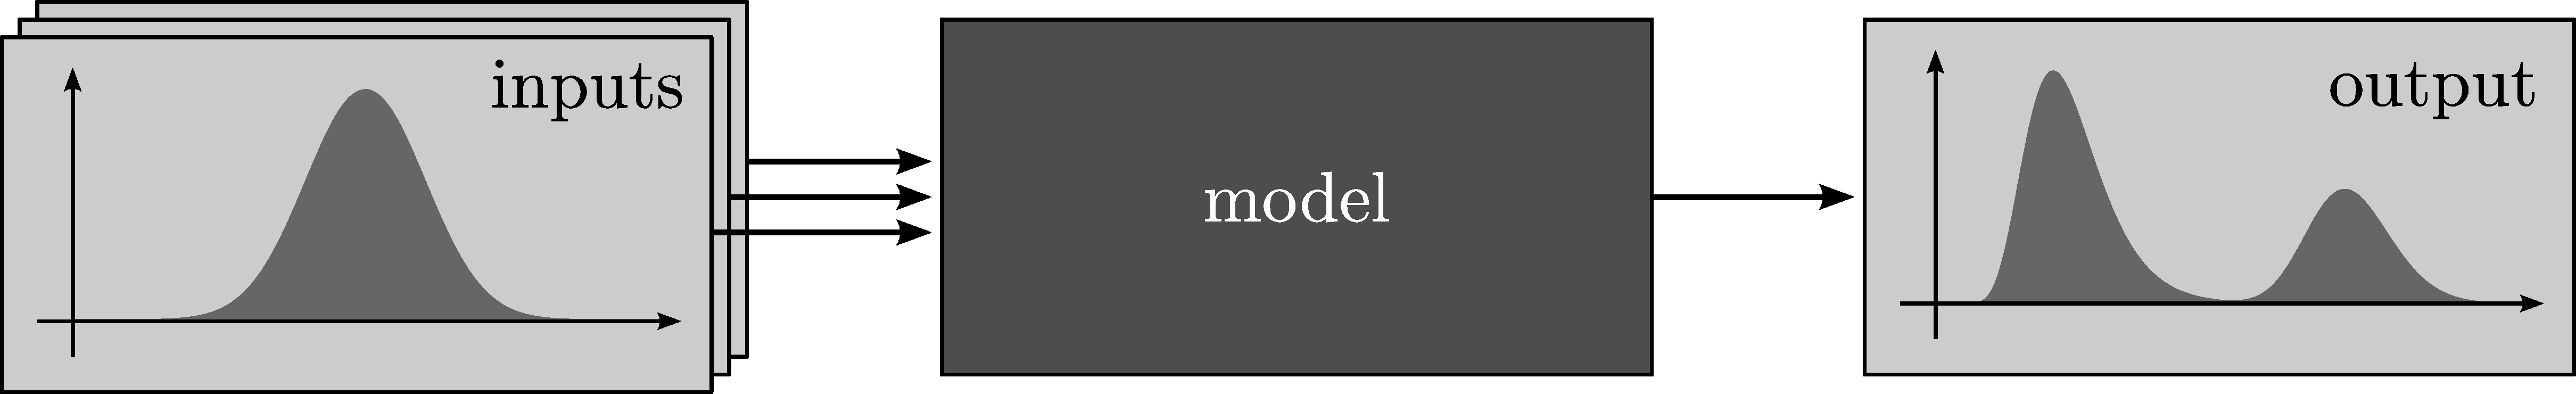
\includegraphics[width=13cm]{fig_UQ_ForwardPropagation}
  \caption[Forward uncertainty propagation]{Forward uncertainty propagation.}
  \label{fig:UQ:ForwardPropagation}
\end{figure}

\subsection{Monte Carlo simulation}
% MONTE CARLO SIMULATION
An appealingly simple approach to compute the first moments of the output distribution is Monte Carlo (MC) simulation.
For \(K \in \mathds{N}_{>1}\) representative input samples \(\mathcal{X} = (\bm{x}^{(1)},\ldots,\bm{x}^{(K)})\),
which are independently drawn from the input distribution in \cref{eq:UQ:InputRV},
one has to compute the corresponding responses \(\mathcal{Y} = (\tilde{y}^{(1)},\ldots,\tilde{y}^{(K)})^\top\).
Here, \(\tilde{y}^{(k)} = \mathcal{M}(\bm{x}^{(k)})\) are realizations of the random variable in \cref{eq:UQ:OutputRV} for \(k = 1,\ldots,K\).
The moments in \cref{eq:UQ:OutputMean,eq:UQ:OutputVariance} can then be estimated via the sample approximations
\begin{equation} \label{eq:UQ:MonteCarloMeanVariance}
  \overline{\mu}_{\tilde{Y}} = \frac{1}{K} \sum\limits_{k=1}^K \tilde{y}^{(k)}, \quad
  \overline{\sigma}_{\tilde{Y}}^2 = \frac{1}{K-1} \sum\limits_{k=1}^K \left( \tilde{y}^{(k)} - \overline{\mu}_{\tilde{Y}} \right)^2.
\end{equation}
\par % DISCUSSION
This is a universal and solid approach to characterize the response distribution.
Because the MC estimates in \cref{eq:UQ:MonteCarloMeanVariance}, provided that at least the first two and four moments respectively exist,
enjoy input dimension--independent convergence rates of the statistical sampling errors with the number of random samples,
they are often used in high-dimensional problems.
Especially for problems of low and moderate dimension, other alternatives might be superior.
A local method based on a Taylor expansion of the model and more global metamodeling techniques are discussed
in \cref{sec:Uncertainty:TaylorApproximation,sec:Uncertainty:SurrogateModeling}, respectively.